%	\noindent \textbf{RQ2:}\textbf{ Can metrics from code, log and developer dimension help in explaining the stability of logs?}
%	\\\\
%\noindent \textbf{Motivation}

From our preliminary analysis, we find that 45\%-55\% of logs are changed in our subject applications. This affects the log processing tools which run on these studied applications, making developers spend more time on maintenance of those tools. In order to identify which metrics can help explain the stability of logs, in the section we construct a random forest classifier and identify the important metrics.

% we build a random forest classifier. 


% Hence, there is a need to identify these non-stable logs to simplify the job of developers. It can also benefit log processing tool developers to develop more robust applications making them more stable.

%
%can be extracted from control versions systems by developersthem.  \\


\subsection{Approach}

We use process and change metrics collected from the code, log developer dimensions to build the classifier. Change metrics measure the changes to the applications at the time of introduction of the log and process metrics measure the source code of the applications. We use the git repository to extract the change metrics and product metrics for the studied applications. Table~\ref{tba:Taxonomy} lists all the metrics we collect for each dimension. We define each metric and the rationale behind the choice of each metric.  We use the product and process metrics because this data can be extracted from control versioning systems (CVS) easily by developers. It also benefits log processing tool developers as they do not need domain knowledge about the application to understand these metrics.\\

%To find the stability of logs in our studied systems, we extract code and log churn metrics from the Git repository and developer metrics from JIRA. We use code churn metrics because prior work has linked logs to development knowledge and issue reports~\cite{IanIcesm}.




%To build prediction models it is necessary to track the changes to logs within the time frame of our study. To achieve this we built a tool which tracks the changes made to each log.  
%
%Since no prior work exists( to our best knowledge ) to predict the stability of logs, we use the code and developer related metrics  to explain the stability of logs. Table ( make table for metrics) explain the different metrics in each category and the rationale for using them. Figure ( make figure explaining process of when log metrics collected and log tracked) shows the process of when metrics are collected and tracking of log. 

%	
%\textbf{Random Forest:} We build random forest to help in predicting the log changes in the revisions of studied systems. A random forest is collection of largely uncorrelated decision trees where they trees combine their results to form a generalized predictor (ref paper). Random forests use bagging strategy (breiman 1996), where the decision trees are constructed using a bootstrap sample dataset. The trees are independent i.e, they do not reply on the earlier trees. In addition to this, random forests split each node using the best among a subset of predictors randomly chosen at that node (breiman 2001). This makes the random forests robust against over-fitting and are more accurate than other tree algorithms (Brieman 2001). 

\noindent{\textbf{{Model construction}}}

We build random forest models to explain the stability of logs in our studied applications. A random forest is a collection of largely uncorrelated decision trees in which the results of all trees are combined to form a generalized predictor~\cite{Albert2008424}. In our model the product and change metrics are the explanatory variables and the dependent class variable is a boolean variable that represents whether the log is changed or not (i.e., '0' for not changed and '1' for changed).

\begin{table*}
	\centering \protect\caption{Taxonomy of metrics considered for model construction}	
	\label{tba:Taxonomy} %
	\begin{tabular}{|c|l|l|>{\raggedright}p{1\columnwidth}|}
		\hline 
		Dimension  & Metrics  & Values  & Definition (d) -- Rationale (r)\tabularnewline
		\hline 
		\hline 
		\multirow{12}{*}{Change Metrics} & 
		Log revision count	 & Numerical &
		d: The number of prior commits which had log changes. \tabularnewline
		\cline{2-4} &  &  &
		r: This helps to identify if the file is prone to log changes.\tabularnewline
		\cline{2-4} &
		Old Log	 & Boolean (0 -1) &
		d: Check if the log is added to the file after creation or it wad added when file was created. \tabularnewline
		\cline{2-4} &  &  &
		r: This helps to identify if the logs added into file after creation are changed more than logs added at creation of file. 	\tabularnewline
		\cline{2-4} &
		Is deleted	 & Boolean (0 -1) &
		d: Check if the log is deleted from the file \tabularnewline
		\cline{2-4} &  &  &
		r: Identify the logs which get deleted in the file after they are added 	\tabularnewline
		\cline{2-4} & 		
		Deleted count & Numerical &
		d: Number of commits from the time a log is introduced into the file till it is deleted (removed) from the file. \tabularnewline
		\cline{2-4} &  &  &
		r: Find out how long it takes before a log is removed from the file. \tabularnewline
		\cline{2-4} 
		& New File & Boolean (0 -1) & 
		d: Check if the log is added in a new file (i.e., newly committed)\tabularnewline
		\cline{2-4} &  &  & 
		r: This helps to identify which logs where added later in subsequent commits.\tabularnewline
		\cline{2-4} 
		& Total revision count & Numerical & d: Total number of commits made to the file before the log is added.
		This value is 0 for logs added in the initial commit but not for logs
		added overtime. \tabularnewline
		\cline{2-4} 
		&  &  & r: This helps to find out if the file is changed heavily which can
		result in log changes~\cite{Characterizinglogs}. \tabularnewline
		\cline{2-4} 
		& Code churn in commit & Numerical & d: The code churn of the commit in which a log is added. \tabularnewline
		\cline{2-4} 
		&  &  & r: Log changes are correlated to code churn in files~\cite{EMSEIAN}. \tabularnewline
		\cline{2-4} 
		& Variables declared & Numerical & d: The number of variables which are declared before the log statement.
		(we limit to 20 lines before log statement).\tabularnewline
		\cline{2-4} 
		&  &  & r: When new variables are declared, developers may log the new variables
		to obtain more information~\cite{Characterizinglogs}. \tabularnewline
		\cline{2-4} 
		& SLOC & Numerical & d: The number of lines of code in the file.\tabularnewline
		\cline{2-4} 
		&  &  & r: Large files have more functionality and are more prone to changes~\cite{zhang2009investigation}
		and more log changes~\cite{Characterizinglogs,EMSEIAN}. \tabularnewline
		\hline 
		\multirow{22}{*}{Product Metrics} & Log context & Categorical & d: Identify the block in which a log is added. (i.e., `if', `if-=else',
		`try-catch', `exception', `throw', `new function').\tabularnewline
		\cline{2-4} 
		&  &  & r: Prior research finds that logs are mostly used in assertion checks,
		logical branching, return value checking, assertion checking~\cite{Fu1}. \tabularnewline
		\cline{2-4} &
		Log change type	 & Boolean (0 -1) &
		d: Check the type of log change the log has undergone before i.e., relocation, text-variable change, level change. \tabularnewline
		\cline{2-4} &  &  &
		r: This helps in removing the relocation changes from the dataset and check if logs that have changed once before undergo similar changes again.  	\tabularnewline
		\cline{2-4} 	
		
		& Log variable count & Numerical & d: Number of variables logged.\tabularnewline
		\cline{2-4} 
		&  &  & r: Over 62\% of logs add new variables~\cite{Characterizinglogs}.
		Hence fewer variables in the initial log statement might result in
		addition later. \tabularnewline
		\cline{2-4} 
		& Log density & Numerical & d: Ratio of number of log lines to the source code lines in the file.\tabularnewline
		\cline{2-4} 
		&  &  & r: Research has found that there is on average one log line per 30
		lines of code~\cite{Characterizinglogs}. If it is less it suggests
		there may be additions in later commits.\tabularnewline
		\cline{2-4} 
		& Log level & Categorical & d: Identify the log level (verbosity) of the added log (i.e., `info',
		`error', `warn', `debug', `trace' and `trace').\tabularnewline
		\cline{2-4} 
		&  &  & r: Developers spend significant amount of time in adjusting the verbosity
		of logs~\cite{Characterizinglogs}. \tabularnewline
		\cline{2-4} 
		& Log text length & Numerical & d: Number of text phrases logged (i.e., we count all text present
		between a pair of quotes as one phrase).\tabularnewline
		\cline{2-4} 
		&  &  & r: Over 45\% of logs have modifications to static context~\cite{Characterizinglogs}.
		Logs with fewer phrases might be subject to changes later to provide
		better explanation.\tabularnewline
		\cline{2-4} 
		& Resolution time & Numerical & d: The time it takes for the issue to get fixed. It is defined as
		the time it takes since an issue is opened until closed. \tabularnewline
		\cline{2-4} 
		&  &  & r: More resolution time might suggest a more complex fix with more
		log churn. \tabularnewline
		\cline{2-4} 
		& Number of developers involved & Numerical & d: Total number of unique developers who contribute to the file.\tabularnewline
		\cline{2-4} 
		&  &  & r: Components with many unique authors likely lack strong ownership, which in turn may lead to more defects~\cite{mcintosh2014impact}
		and change logs~\cite{EMSEIAN}. \tabularnewline
		\cline{2-4} 
%		& Number of comments & Numerical & d: Total number of discussion posts on the issue. \tabularnewline
%		\cline{2-4} 
%		&  &  & r: Number of comments is correlated to the resolution time of issue
%		reports~\cite{giger2010predicting}. More comments may also indicate
%		the issue is more complex resulting in more code churn and log changes. \tabularnewline
%		\cline{2-4} 
%		& Developer experience & Numerical & d: The number of commits the developer has made prior to this commit. \tabularnewline
%		\cline{2-4} 
%		&  &  & r: Research has shown that experienced developers might take up more
%		complex issues~\cite{rahman2011ownership} and therefore may leverage
%		logs more~\cite{EMSEIAN}. \tabularnewline
%		\cline{2-4} 
%		& Issue type  & Categorical & d: Identify the type of issue, i.e., `Bug', `Improvement', `Task',
%		`New Feature', `Sub-Task', `Test'. \tabularnewline
%		\cline{2-4} 
%		&  &  & r: Some issue types might have higher code churn than others (example:
%		Bug and New features might have more code churn when compared to Sub-Tasks)
%		and are committed faster.\tabularnewline
%		\cline{2-4} 
%		& Priority type & Categorical & d: Identify the priority of the issue i.e., `Critical', `Blocker',
%		`Major', `Minor' and `Trivial'\tabularnewline
%		\cline{2-4} 
%		&  &  & r: Research has shown that priority of issue affects resolution time
%		of bug fixes~\cite{MarkFixTime}. A Higher priority indicates the
%		issue will be fixed faster with log changes. \tabularnewline
%		\cline{2-4} 
		& File ownership  & Numerical (0-1) & d: Identify the percentage of the file written by developer introducing the log \tabularnewline
		\cline{2-4} 
		&  &  & r: The owner of the file is more likely to introduce stable logs than developers who have not edited the file before. \tabularnewline
		\hline 
	\end{tabular}\protect
\end{table*}

\begin{figure}
	\centering
	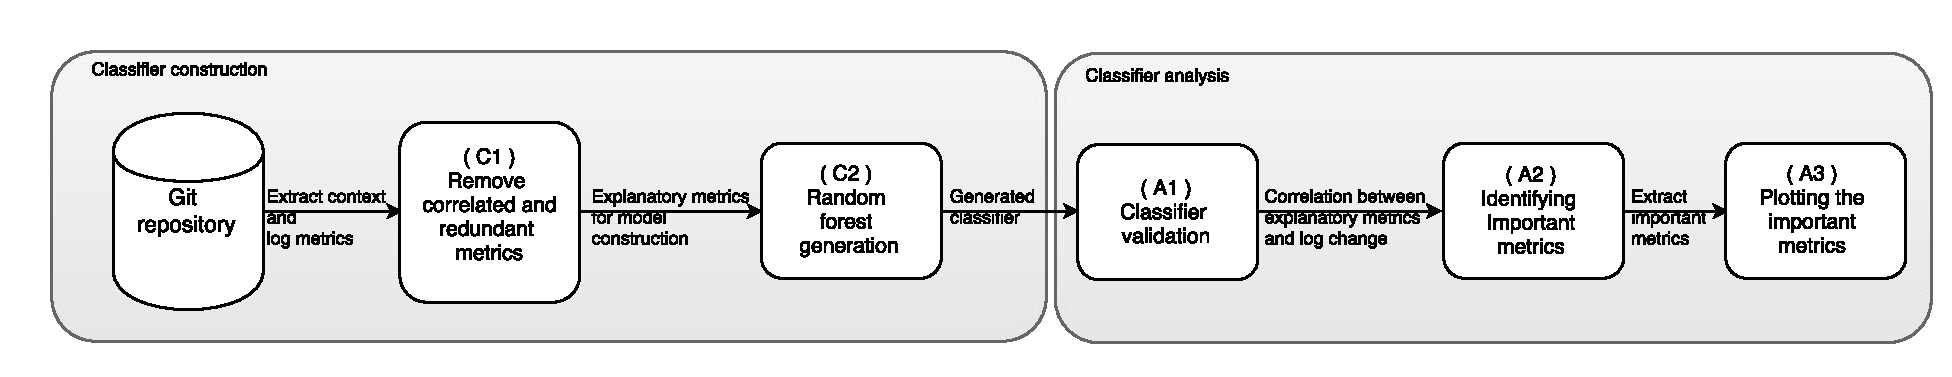
\includegraphics[width=1\columnwidth]{ModelCreationLogGeanology}
	\caption{Overview of Model construction(C) and flow of data in random forest generation}
	\label{fig:ModelCreationLogGeanology}
\end{figure}  


Figure~\ref{fig:ModelCreationLogGeanology} provides an overview of the four construction steps (C1 to C4) for building a random forest model and evaluating the model. We adopt the statistical tool R to model our data and use the `RandomForest' package to generate the random forests.\\

\textbf{\textsl{(C1 - Correlation analysis) }}

Correlation analysis is necessary to remove the highly correlated metrics from our dataset. Collinearity between metrics can affect the performance of a model because, small changes in one metric can affect the values of other metrics causing large changes on the dependent class variable.

 We use Spearman rank correlation~\cite{spearmanbook} to remove these correlated metrics from our data. Spearman rank correlation assesses how well two metrics can be described by a monotonic function. We use Spearman rank correlation instead of Pearson~\cite{pearsonbook} because Spearman is resilient to data that is not normally distributed. We use the function `varclus' in R to perform the correlation analysis.

Figure~\ref{fig:SpearmanActiveMQ} shows the hierarchically clustered Spearman $\rho $ values in the ActiveMQ project. The solid horizontal lines indicate the correlation value of the two metrics that are connected by the vertical branches that descend from it.  We include one metric from the sub-hierarchies which have correlation $|\rho| > 0.7 $. The gray line indicates our cutoff value ($ | \rho | $ = 0.7). We use cutoff value of ($ | \rho | $ = 0.7) as used by prior research~\cite{ShaneOLS} to remove the correlated metrics before building our model. \\




\begin{figure}
	\centering
	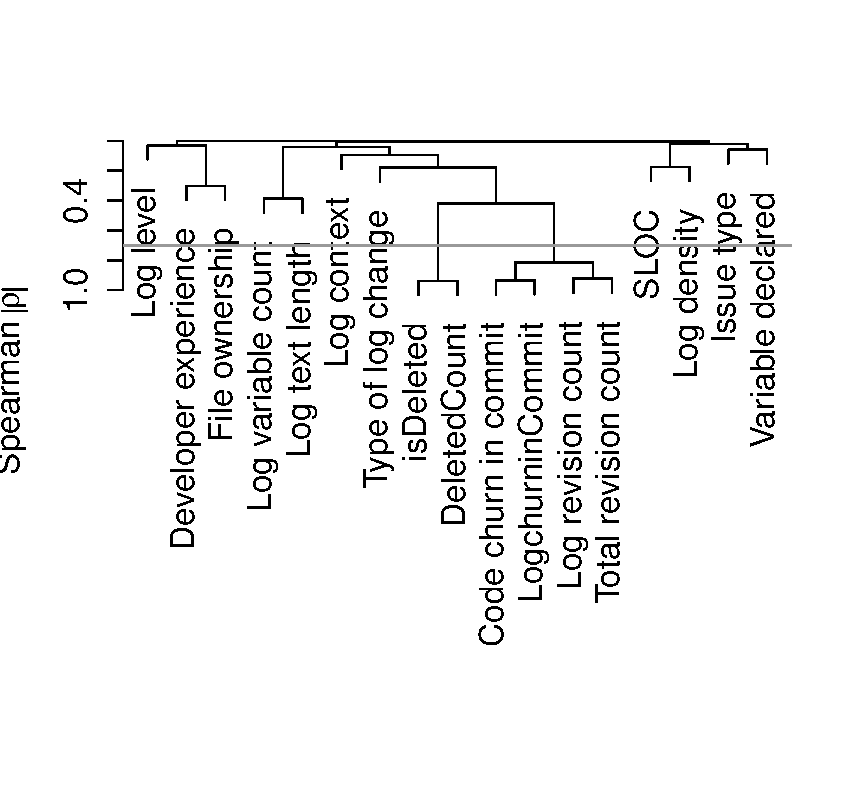
\includegraphics[height=1\columnwidth,width=0.9\columnwidth]{SpearmanActiveMQ}
 \vspace*{-1cm}	\caption{Hierarchical clustering of variables according to Spearman’s $\rho$ in ActiveMQ}
	\label{fig:SpearmanActiveMQ}
\end{figure}


\textbf{\noindent\textsl{(C2 - Random forest generation)}}

After we eliminate the correlated metrics from our datasets, we construct the random forest model. Random forest is a black-box ensemble classifier, which operates by constructing a multitude of decision trees on the training set and uses this to classify the testing set.
\begin{figure}
	\centering
	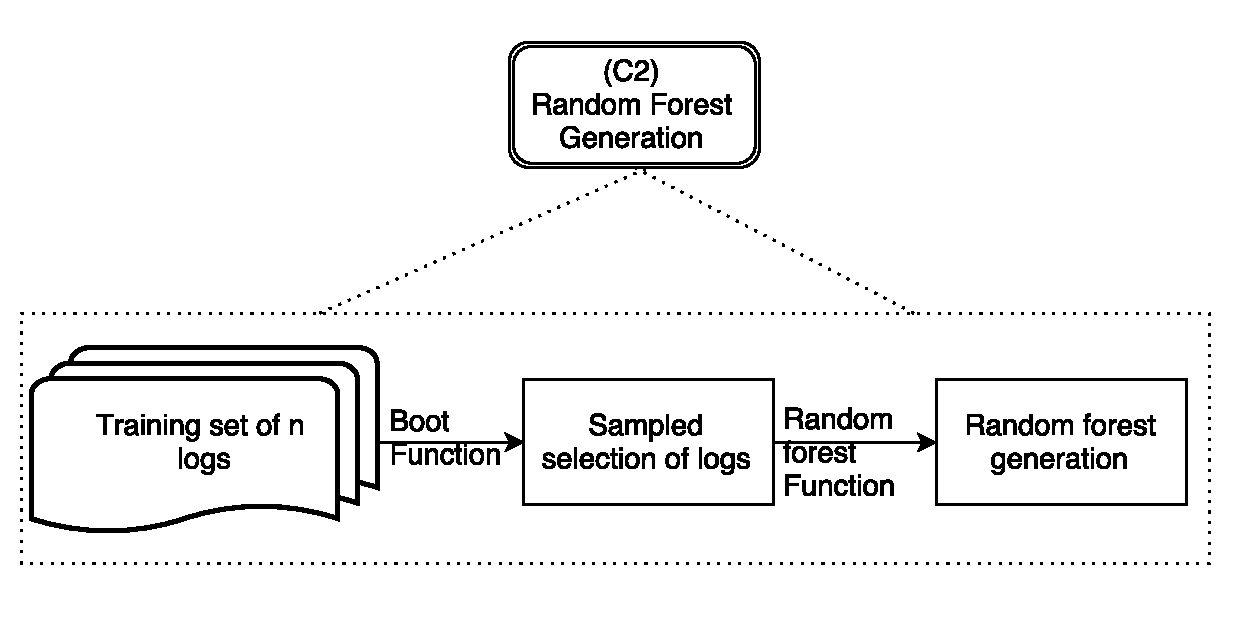
\includegraphics[height=.7\columnwidth,width=1\columnwidth]{BootRandomForest}
	\caption{ Overview of random forest generation in C2}
	\label{fig:BootRF}
\end{figure}


Given a dataset of \textsl{m} logs for training, $ D = \{ (X_{1}Y_{1}),...,(X_{m}Y_{m}) \} $ where $X_{i, i = 1...m}$, is a vector of descriptors (i.e., $X$ are the metrics which are left after correlation analysis ) and $Y_{i}$ is the flag which indicates whether a log is changed or not. Figure~\ref{fig:BootRF} explains the construction of the random forest classifier and the steps are explained below.
\begin{enumerate}
\item From the training set of \textsl{m} logs, a random sample of \emph{n} components is selected with replacement (i.e., bootstrap sample)~\cite{ShaneOLS}.

We use the `boot' function from the `boot' package in R to generate bootstrap samples. The boot function generates a set of random indices, with replacement from the integers 1:\emph{n}.

\item From the sampled selection, many classification trees are grown without pruning. Each classification tree gives a vote, i.e., `true' if log is changed and `false' if not. The random forest chooses the class with most number of votes over all the trees in the forest. This strategy helps to make the random forests more robust against over-fitting~\cite{breiman1996bagging}.

 We use the `randomForest' function from the `randomForest' package in R to generate the random forest model. 


\item The above steps are repeated until \textsl{M} such models are grown.
\item Predict new data by aggregating the prediction of the $M$ models generated.
\end{enumerate}  

\begin{table}[t]
	\centering
		\caption{Confusion Matrix}
		\label{tba:confusion}
	\begin{tabular}{|ll|l|l|}
		\cline{1-4}
		&                 & \multicolumn{2}{c|}{Predicted}            \\ \cline{3-4} 
		&                 & Log changed         & Log not changed     \\ \hline
		\multicolumn{1}{|c|}{\multirow{2}{*}{Actual}} & Log change      & True positive (TP)  & False negative (FN) \\ \cline{2-2} 
		\multicolumn{1}{|c|}{}                        & Log not changed & False positive (FP) & True negative (TN)  \\ \hline
	\end{tabular}
		

\end{table}

%\begin{table}[t]
%
%	\begin{tabular}{|>{\raggedright}p{0.1\columnwidth}>{\raggedright}p{0.2\columnwidth}|l>{\raggedright}p{0.2\columnwidth}|}
%		\hline 
%		\multicolumn{1}{|>{\raggedright}p{0.03\columnwidth}}{\multirow{2}{0.03\columnwidth}{}} &  & \multicolumn{2}{c|}{Predicted}\tabularnewline
%		&  & Log has changed & Log has not-changed\tabularnewline
%		\hline 
%		\multirow{2}{0.03\columnwidth}{Actual} & Log has changed  & TP (True Positive)  & FN (False Negative ) \tabularnewline
%		& Log has not-Changed  & FP (False Positive )  & TN (True Negative) \tabularnewline
%		\hline 
%	\end{tabular}\protect
%	
%	
%
%\end{table}

\textbf{
\noindent \textsl{(C3 - Model evaluation)}}

After we build the random forest model, we evaluate the performance of our model using precision, recall, F-measure and Brier Score. These measures are functions of the confusion matrix as shown in Table~\ref{tba:confusion} and are explained below.

\textsl{Precision (P)} measures the correctness of our model in predicting which log will undergo a change in the future. It is defined as the number of logs which were accurately predicted as changed over all logs predicted to have changed as explained in Equation~\ref{f:precision}.   \\
	 \begin{equation}
 P =  \dfrac{TP}{TP + FP } 
 \label{f:precision}
	 \end{equation}	
	 
\textsl{Recall (R)} measures the completeness of our model. A model is said to be complete if the model can predict all the logs which will get changed in our dataset. It is defined as the number of logs which were accurately predicted as changed over all logs which actually change as explained in Equation~\ref{f:recall}.
	 \begin{equation}
	 R =  \dfrac{TP}{TP + FN } 
	 \label{f:recall}
	 \end{equation}	
	 
\textsl{F-Measure} is the harmonic mean of precision and recall, combining the inversely related measure into a single descriptive statistic as shown in Equation~\ref{f:Fmeasure}~\cite{F-Measure}.
	 \begin{equation}
	 F =  \dfrac{2 \times P \times R}{P + R } 
	 \label{f:Fmeasure}
	 \end{equation}	
	 
\textsl{Brier Score (BS)} is a measure of the accuracy of the predictions in our model~\cite{wilks2011statistical}. It explains how well the model performs compared to random guessing i.e.,  a perfect classifier  will have Brier score of 0 and perfect misfit classifier will have Brier score of 1 (predicts probability of log change when log not changed). This means the lower the Brier score value, the better our random forest classifier.
%As the Brier score measure the total difference between the event and the forecast probability of the event, 
 
%The most common formulation of Brier Score is shown in Equation~\ref{f:BS}, where $f_{t}$ is the probability that was predicted, $o_{t}$ is the actual outcome of the event at the instance $t$ (0 if log is not changed and 1 if it is changed), and $N$ is the number of forecasting instances. 

%If the predicted value is 70\% and the log is changed, the Brier Score is 0.09 (lower the Brier score, the more likely the event will occur). It reaches 0.25 

%	 \begin{equation}
%	 BS =  \dfrac{1}{N}\Sigma_{t=1}^{N} (f_{t} - o_{t} )^{2} 
%	 \label{f:BS}
%	 \end{equation}	

These performance measure, described previously only provide insight into how the random forest models fit the observed dataset, but it may overestimate the performance of the model if the model is over-fit.

To account for the overfitting in our models, we use \textsl{optimism} measure, as used by prior research~\cite{ShaneOLS}. The \textsl{optimism} of the performance measures are calculated as follows.
\begin{enumerate}
	\item From the original dataset with \textsl{m} records, select a bootstrap sample with \textsl{m} components with replacement.
	\item Build random forest as described in (C2) using the bootstrap sample.
	\item Apply the classier model built from bootstrap sample on both the bootstrap and original data sample, calculating precision, recall, F-measure and Brier score for both data samples.
	\item Calculate \textsl{Optimism} by subtracting the performance measures of the bootstrap sample against the original sample. 	
\end{enumerate}

	The above process is repeated 1,000 times and the average (mean) \textsl{optimism} is calculated. Finally, we calculate \textsl{optimism-reduced} performance measures for precision, recall, F-measure and Brier score by subtracting the averaged optimism of each measure, from their corresponding original measure.  The smaller the optimism values, the more stable the original model fit is.
	\\

\textbf{\noindent \textsl{(C4 - Importance of each metric in relation to log stability)}}
To find the importance of each metric in a random forest model, we use a permutation test. In this test, the model built using the bootstrap data (i.e., two thirds of the original data) is applied to the test data (i.e., remaining one third of the original data).  

Then, the values of the $X_{i}$ $^{th}$ metric of which we want to find importance for, are randomly permuted in the test dataset and the accuracy of the model is recomputed. The decrease in accuracy as a result of this permutation is averaged over all trees, and is used as a measure of the importance of metric $X_{i}$th in the random forest.

We use the `importance' function defined in `RandomForest' package of R, to calculate the importance of each metric. We call the `importance' function each time during the bootstrapping process to obtain 1000 importance scores for each metric in our dataset. 	

As we obtain 1000 data sets for each metric because of bootstrapping process, we use the \textbf{Scott-Knott} (SK) clustering to group the metric based on their means~\cite{Cluster1,Cluster2}. This is done to group metrics which are strong predictors of likelihood of log change. The SK algorithm uses the hierarchical clustering approach to divide the metrics and uses the likelihood ratio test to judge the difference between the groups. This assures the means of metrics within a group not to be statistically significantly different. We use the `SK' function in the `ScottKnott' package of R and set the significance threshold parameter to 0.05 to cluster the metrics into different groups. 
%\begin{table}

%	\centering

\begin{figure}[tb]
	
	\centering
	\subfloat{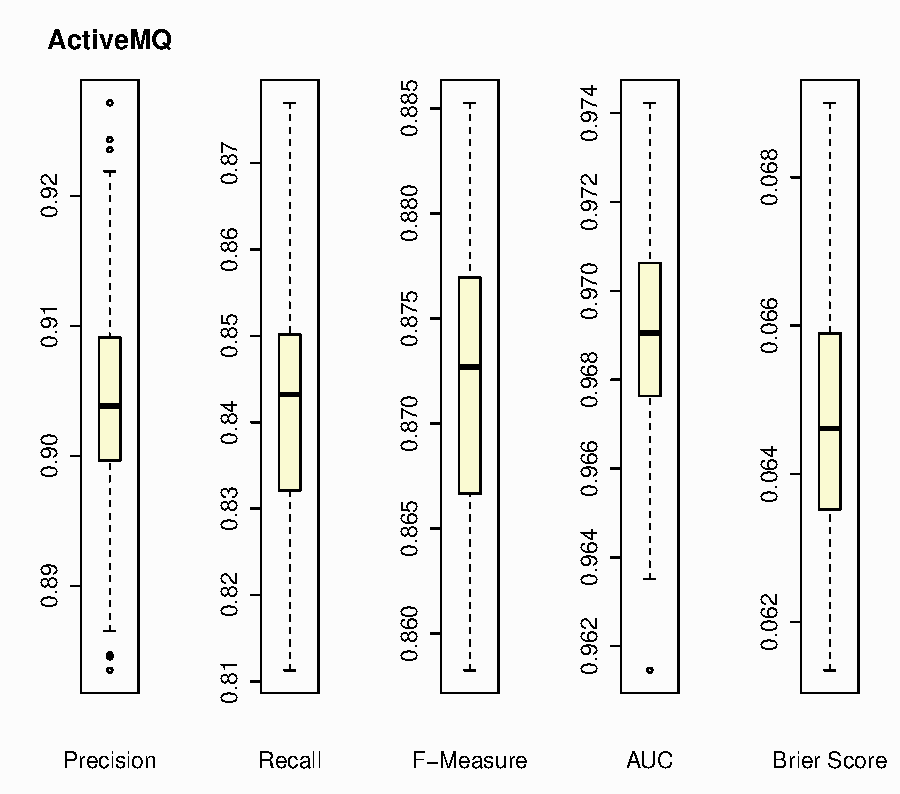
\includegraphics[width=0.49\columnwidth]{ActiveMQResults}\label{fig:f4}}
	\hfill
	\centering
	\subfloat{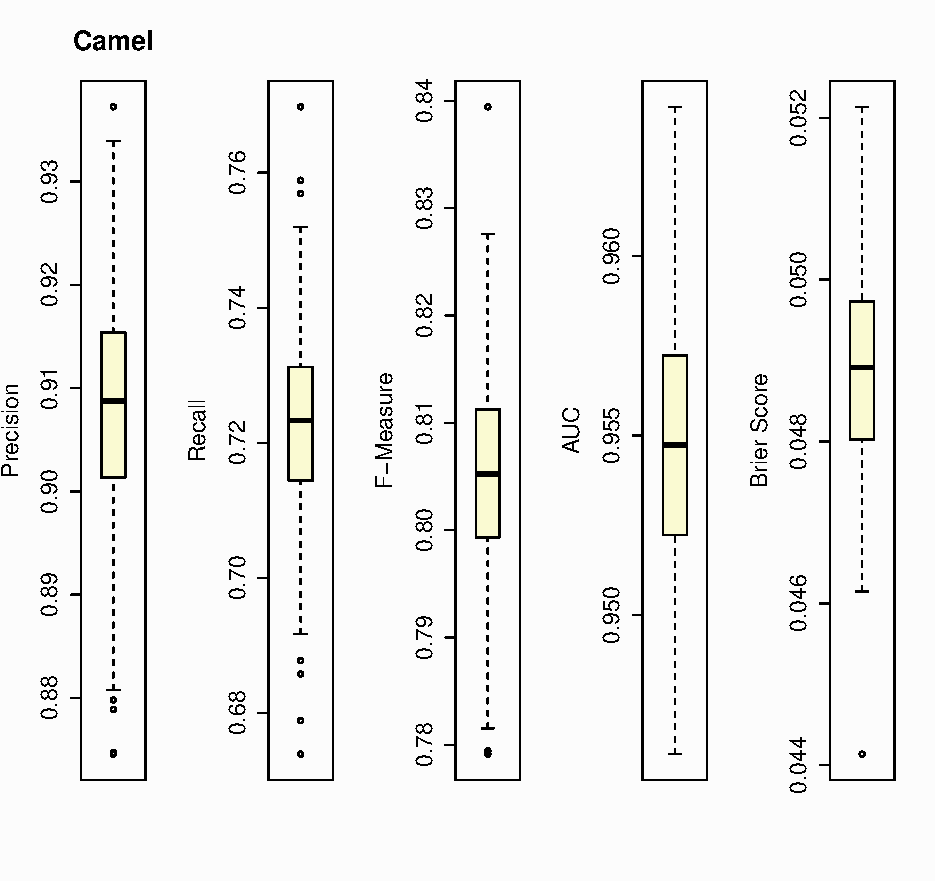
\includegraphics[width=0.49\columnwidth]{CamelResults} }
	\hfill
		\centering
		\subfloat{\includegraphics[width=0.49\columnwidth]{CloudStackResults}
			\label{fig:f4}}
		\hfill
			\centering
			\subfloat{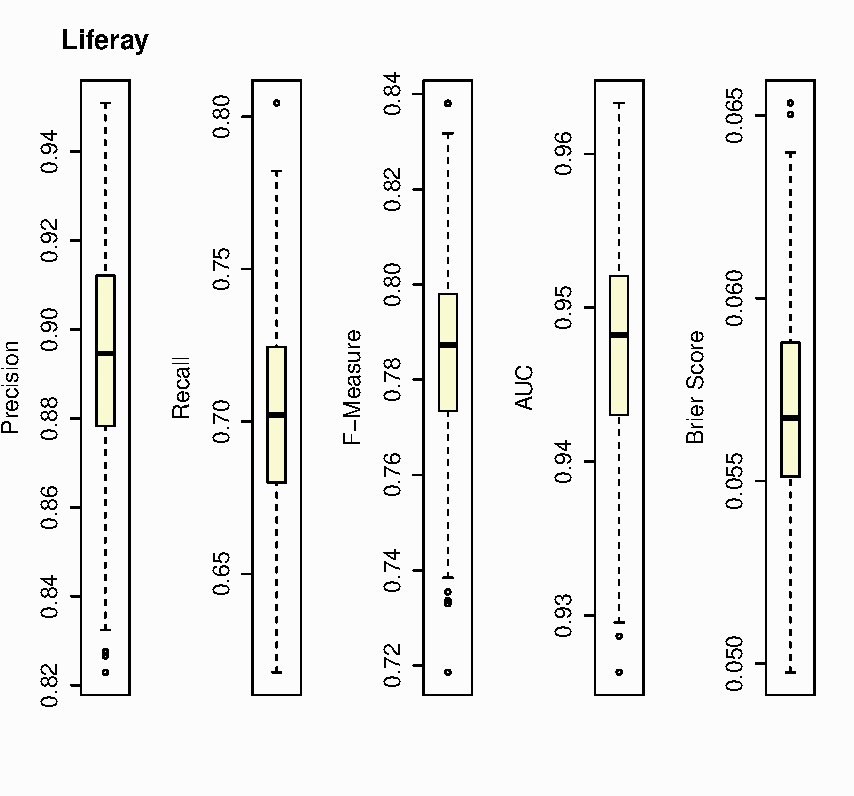
\includegraphics[width=0.49\columnwidth]{LiferayResults}\label{fig:f4}}
			\hfill
%	\caption{Distribution of the number of developers responsible for changing a log}
		\caption{The optimism reduced performance measures of the four projects}
	\label{fig:optmisim}

\end{figure}


%\label{tba:optmisim}
%\end{table}


\subsection{Results}
\begin{table*}[t]
	\protect\protect\caption{The importance values of the metrics (top 10), divided into homogeneous
		groups by Scott-Knott clustering. The `+' and `-' signs signifing positive
		and negative correlation of the metric on log stability. }
	
	\centering
	
	\begin{tabular}{|lll|lll|}
		\hline 
		& \textbf{ Active MQ}  &  &  & \textbf{Camel}  & \tabularnewline
		\hline 
		\textbf{Rank}  & \textbf{Factors}  & \textbf{Importance}  & \textbf{Rank}  & \textbf{Factors}  & \textbf{Importance} \tabularnewline
		\hline 
		1  & SLOC & 0.174 +  & 1  & Ownership of file & 0.207 + \tabularnewline
		2  & Ownership of file & 0.162 +  & 2  & Log density  & 0.175 - \tabularnewline
		& Log variable count & 0.161 +  &   & Developer experience & 0.174 - \tabularnewline
		3 & Developer experience & 0.140 +  & 3  & SLOC & 0.168 + \tabularnewline
		4  & Log density & 0.120 -  & 4 & Log variable count & 0.124 + \tabularnewline
		5  & Variable Declared  & 0.090 -  & 5  & Log level & 0.116 - \tabularnewline
		6  & Deleted count & 0.082 -  & 6  & Elapsed time & 0.109 - \tabularnewline
		7  & Log level & 0.078 -  &   & Issue type & 0.108 + \tabularnewline
		8  & Log churn in commit & 0.060 +  &   & Variable Declared  & 0.108 + \tabularnewline
		\hline 
	\end{tabular}
	\centering
	\begin{tabular}{|lll|lll|}
		\hline 
		& \textbf{CloudStack}  &  &  & \textbf{Life Ray}  & \tabularnewline
		\hline 
		\hline 
		\textbf{Rank}  & \textbf{Factors}  & \textbf{Importance}  & \textbf{Rank}  & \textbf{Factors}  & \textbf{Importance} \tabularnewline
		\hline 
		1  & Code churn in commit & 0.138 +  & 1  & Log density  & 0.152 - \tabularnewline
		2 & Ownership of file & 0.136 +  & 2  & Ownership of file & 0.137 - \tabularnewline
		& Developer experience & 0.135 -  &  & Developer experience & 0.137 + \tabularnewline
		1  & Log density  & 0.122 -  & 3 & SLOC & 0.127 + \tabularnewline
		2  & SLOC & 0.122 +  & 4  & Issue Id & 0.096 - \tabularnewline
		3  & Log variable count & 0.113 +  & 5  & Variable Declared  & 0.093 + \tabularnewline
		1  & Log text length & 0.102 +  &   & Log variable count & 0.091 + \tabularnewline
		2  & Variable Declared  & 0.076 +  & 6  & Log level & 0.081 - \tabularnewline
		3  & Type of log change & 0.063 +  & 7 & Elapsed time & 0.072 +\tabularnewline
		\hline 
	\end{tabular} \label{tba:Scott} 
\end{table*}


\textbf{The random forest classifier achieves a precision of 0.89-0.91 and recall of 0.71-0.91 for our studied applications.} Figure~\ref{fig:optmisim} shows the optimism-reduced values of \textsl{precision}, \emph{recall}, \emph{F-measure} and \emph{Brier score} for each project. The model achieves AUC of 0.95-0.96 across the studied applications. We find the recall of the random forest classier in Liferay is not as high as the other projects. This may be because Liferay has the lowest total number of log lines and close to 50\% of the log changes are log relocations as seen in Table~\ref{tba:logtype}. Because of the lower percentage of logs which are changed, the random forest classifier has fewer nodes (trees) and likelihood of false negatives is higher. 

%lowest percentage of logs which are changed at 20\%, compared to 45-70\% in the other projects. Because of the lower percentage of logs which are changed, the random forest classifier has fewer nodes (trees) and likelihood of false negatives is higher. 

\textbf{The random forest classifier outperforms random guessing.} The classifier achieves Brier scores between 0.04 and 0.07 across all projects. If the model achieves a Brier score of 0.07, it means our model can forecast with 73\% probability a log will change. Brier score reaches 0.25 for random guessing (i.e., predicted value is 50\%).


\subsection*{\textbf{Important metrics for log stability}}

%From Table~\ref{tba:Scott} we see that `file ownership', `SLOC', `log density', and `developer experience' are common across all the projects in our studied systems. 

%The high importance of \emph{SLOC}, \emph{code churn in commit} and \emph{\# of comments} indicate that log stability 

%% LyX 2.1.2 created this file.  For more info, see http://www.lyx.org/.
%% Do not edit unless you really know what you are doing.

\textbf{We find that \emph{log density} is an important metric in our studied applications as shown in Table~\ref{tba:Scott}}. We find that log density has negative correlation with log stability (i.e., increase in log density decreases probability of log change), in all the studied applications. This suggests that when source code is well logged i.e., more logs per lines of code, the logs may communicate the necessary information making them more stable.

\textbf{We find \emph{log variable count} has a positive correlation with log stability as shown in Table~\ref{tba:Scott}}. This implies that more variables in a log results in a higher likelihood that a log will be changed. This may be because there are inconsistencies between logs and the actual needed information intended as shown by prior research~\cite{Characterizinglogs} and developers have to update logs to resolve the inconsistencies.


%\textbf{We find that \emph{SLOC}(source lines of code) is a strong predictor of log change across all projects.} \emph{SLOC} has a positive correlation suggesting that logs in larger files have higher a likelihood of getting changed. 

%We find that \emph{Variable declared} has positive correlation in three of the studied systems, which suggests that when developers add new variables in the commit there is a higher likelihood of log change as they may add or modify the log to output the new data.
%, logs around those comments are less likely to get changed. 


\textbf{We find that \emph{file ownership} is a strong predictor of log change and has positive correlation in three of the studied applications.} This suggests that logs introduced by developers who have little ownership are more unstable and have to be changed. This is seen Figure~\ref{fig:ChangedvsUnchangedlogs}, where in three of the studied applications, the logs which change are introduced by developers who have lower ownership of a file. 

\textbf{We find that \emph{developer experience} has negative correlation in the studied applications.} Even though ActiveMQ and Liferay has positive correlation in Table~\ref{tba:Scott}, we find that these projects have strong code ownership and  two developer are responsible for over 50\% of the total commits within the projects. To remove this strong ownership, we exclude the log changes made by these top developers in ActiveMQ and Liferay and we find that developer experience has negative correlation in both ActiveMQ and Liferay. This suggests that logs which are introduced by more experienced developers are less likely to change in all of the studied applications. 

% is also a strong predictor of log change in all our models but the correlation is split within the projects. We find that in Cloudstack and Camel, developer experience has a negative correlation on log change, where as in ActiveMQ and Liferay developer experience has positive correlation. 
%The positive correlation may be because of strong code ownership seen ActiveMQ and liferay where two developer are responsible for over 50\% of the total commits within the projects. To remove this strong ownership, we exclude the log changes made by these top developers in ActiveMQ and Liferay and we find that developer experience has positive correlation in ActiveMQ. This suggests that logs which are introduced by more experienced developers are less likely to change in three of the studied systems. 

 

%We find that positive correlation might be due strong code ownership in ActiveMQ and Liferay where two developers are responsible for over 50\% of the total commits, within these projects. The negative effect in ActiveMQ and Cloudstack suggests that logs written by more experienced developers are less likely to be changed. 



% This suggests that either (1) more experienced developers have logged the file increasing the stability of the logs or (2) less experienced developers have logged the file making logs unstable. 
%
%In these systems we find that, more logs are introduced by developers with less experience than developers greater experience. 


%This may be because (1) logs that are added by less experience developers are less stable or (2) more experienced developers might not be as careful about logging as new developers.

 

%
% This implies that logs introduced by more experienced developers and are more likely to be changed.  This may be because the experienced developers may be more complacent than less experienced developers, who thoroughly log the code. 

%We find that other metrics from the developer dimension are not consistent among the studied systems. This may be because each project might have different philosophy of development, for example we find that \emph{resolution time} has negative effect in Liferay and Camel but has positive effect in ActiveMQ. This suggests that logs are more likely to change in ActiveMQ when the resolution time of issue increases, but less likely in Liferay and Camel. 


\hypobox {Our Random Forest classifier achieves a precision of 89\%-91\% and recall of 71\%-91\% across all studied applications. We find file ownership, SLOC, developer experience and log density to be strong predictors of log change in our studied applications.}






